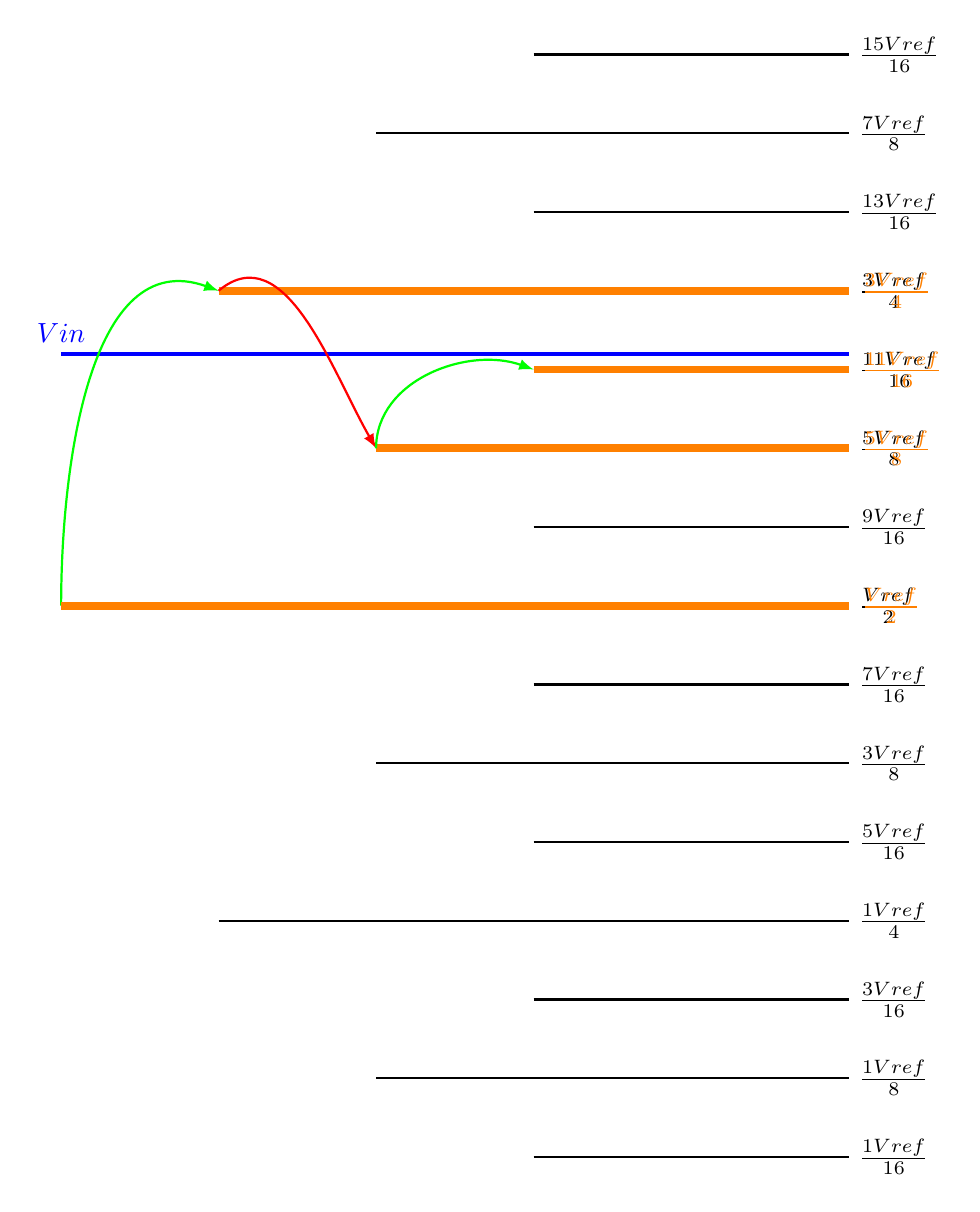
\begin{tikzpicture}
 \draw[thick] (0, 0) --++ (10,0) node[right]{$\frac{V\subb{ref}}{2}$};
 \draw[thick] (2, 4) --++ (8,0) node[right]{$\frac{3V\subb{ref}}{4}$};
 \draw[thick] (2,-4) --++ (8,0) node[right]{$\frac{1V\subb{ref}}{4}$};
 \draw[thick] (4, 6) --++ (6,0) node[right]{$\frac{7V\subb{ref}}{8}$};
 \draw[thick] (4,-6) --++ (6,0) node[right]{$\frac{1V\subb{ref}}{8}$};
 \draw[thick] (4,-2) --++ (6,0) node[right]{$\frac{3V\subb{ref}}{8}$};
 \draw[thick] (4, 2) --++ (6,0) node[right]{$\frac{5V\subb{ref}}{8}$};
 \draw[thick] (6, 1) --++ (4,0)  node[right]{$\frac{9V\subb{ref}}{16}$};
 \draw[thick] (6, 3) --++ (4,0)  node[right]{$\frac{11V\subb{ref}}{16}$};
 \draw[thick] (6, 5) --++ (4,0)  node[right]{$\frac{13V\subb{ref}}{16}$};
 \draw[thick] (6, 7) --++ (4,0)  node[right]{$\frac{15V\subb{ref}}{16}$};
 \draw[thick] (6, -1) --++ (4,0) node[right]{$\frac{7V\subb{ref}}{16}$};
 \draw[thick] (6, -3) --++ (4,0) node[right]{$\frac{5V\subb{ref}}{16}$};
 \draw[thick] (6, -5) --++ (4,0) node[right]{$\frac{3V\subb{ref}}{16}$};
 \draw[thick] (6, -7) --++ (4,0) node[right]{$\frac{1V\subb{ref}}{16}$};
 \draw[line width = 0.05cm, blue] (10, 3.2) --++(-10,0) node[above] {$V\subb{in}$};
 \visible<2->{\draw[-latex, thick, green] (0,0) to[out=90, in=160] (2,4);}
 \visible<2>{\draw[line width=0.1cm, orange] (0, 0) --++ (10,0) node[right]{$\frac{V\subb{ref}}{2}$};}
 \visible<3>{\draw[line width=0.1cm, orange] (2, 4) --++ (8,0) node[right]{$\frac{3V\subb{ref}}{4}$};}
 \visible<4>{\draw[line width=0.1cm, orange] (4, 2) --++ (6,0) node[right]{$\frac{5V\subb{ref}}{8}$};}
 \visible<5>{\draw[line width=0.1cm, orange] (6, 3) --++ (4,0) node[right]{$\frac{11V\subb{ref}}{16}$};}
 \visible<3->{\draw[-latex, thick, red] (2,4) to[out=40, in=120] (4,2);}
 \visible<4->{\draw[-latex, thick, green] (4,2) to[out=90, in=160] (6,3);}
\end{tikzpicture}
